\section{BanditMF}
In this section, we will implement the BanditMF proposed in Section 3.4 and compare the experimental results obtained using different multi-armed bandit algorithms according to different criteria. In this experiment, the \textit{$\epsilon$-greedy}, \textit{UCB}, and \textit{Thompson sampling} algorithms will be used.We will implement BanditMF's process one by one as follows.

\textbf{\textit{Dataset}}. MovieLens will be used in this experiment, which contains the same data as we described in the last two experiments.

\textbf{\textit{Matrix factorization}}.  For BanditMF we use the bias method to implement matrix factorization, where $\hat{\boldsymbol{r}}_{u,i}=b_{u,i}+q_{i}^{T} p_{u}$ and $b_{u,i}$ is the combination of user bias, item bias, and average rating.

For the result shown in Figure 4.24, we generate a predicted user-item rating matrix with a size of 610 $\times$ 9724 
\begin{figure}[htbp]
    \centering
    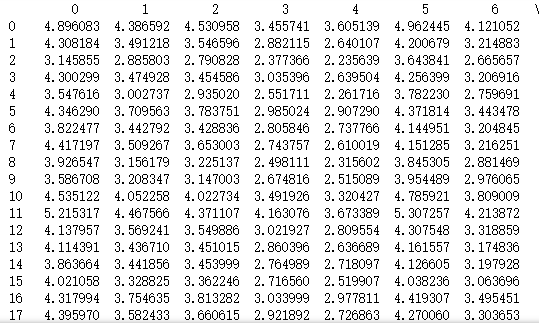
\includegraphics[scale=0.8]{figure/ex1.png}
    \caption{Partial of user-item predicted matrix }
\end{figure}

\textbf{\textit{Clustering}}. We perform the clustering on the row of the predicted user-item rating matrix $\hat{R}$, which means that we cluster the users who share similar rating preferences. In this experiment, we adopt a machine learning algorithm library called \textit{scikit-learn}. Based on the library, \textit{K-means} algorithm is adopted, which is measured by \textit{Euclidean distance}. We set the parameter \textit{n\_clusters}$=$3, which means that we will cluster all users into three clusters. Also, we set the value of parameter \textit{n\_init} to 20, which means that the \textit{K-means} algorithm will be run with 20 different centroid seeds and output the best result in 20 consecutive runs as the final result. Figure 4.25 shows the above iterations. As the number of iterations increases (i.e., x-axis), the sum of the Euclidean distances decreases (i.e., y-axis).

\begin{figure}[htbp]
    \centering
    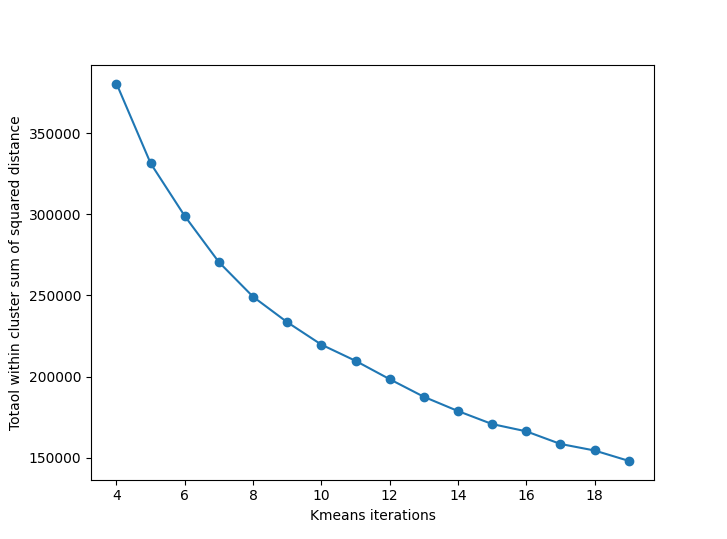
\includegraphics[scale=0.6]{figure/clu1.png}
    \caption{Iterations of K-means}
\end{figure}

Finally, by clustering, we got a 3 $\times$ 9724 predicted user-item rating matrix, shown in Figure 4.26, which means that we converted the original 610 $\times$ 9724 predicted user-item rating matrix to the 3 $\times$ 9724 clustered user-item rating matrix.
\begin{figure}[htbp]
    \centering
    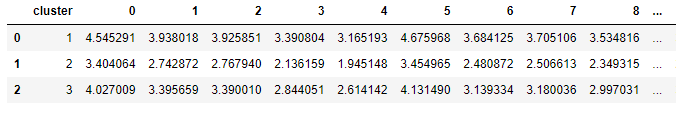
\includegraphics[scale=0.6]{figure/exs4.png}
    \caption{Predicted user-item rating matrix after clustering}
\end{figure}

\textbf{\textit{Online recommendation module}}.In the online recommendation, we used three different multi-armed bandit algorithms for the comparison, including \textit{$\epsilon$-greedy}, \textit{UCB}, and \textit{Thompson sampling}. The bandit algorithm takes the clustered predicted user-item rating matrix as data, and then selects and recommends items to the target users. After receiving the user's rating, the reward and regret are calculated. Then judge whether the user is still a cold user. If so, continue to update the Bandit algorithm with the received data; if not, transfer the user to the offline system and append the user-item rating matrix.

\textbf{\textit{Evaluation criteria}}. In addition to the \textit{rewards} and \textit{regrets} which are the common criteria in the multi-armed bandit algorithm, we have introduced two new criteria: \textit{discounted cumulative gain} (DCG) and \textit{normalized discounted cumulative gain} (NDCG) \cite{ndcg}. Their formulas are shown below:
\begin{equation}
    D C G(u)=r_{u, 1}+\sum_{t=2}^{T} \frac{r_{u, t}}{\log _{2} t}
\end{equation}
\begin{equation}
    N D C G=\frac{1}{N} \sum_{u} \frac{D C G(u)}{D C G^{*}(u)}
\end{equation}
We can see from the formula that these two criteria will discount the reward at a later stage, which means that the accuracy (i.e., user satisfaction) of early recommendations is more important than that of late recommendations, which is why these two criteria are applied here. Since we focus on solving the user's cold start problem, we need the algorithm to make accurate recommendations in a shorter period of time. However, when the user is no longer a cold user, accurate recommendations lose value because the user may give up using the server before you can make accurate recommendations.

\textbf{\textit{Result}}. We use $T$ to denote the total rounds, and $N$ denotes the number of new users. Further, $R_{t}$ represent the cumulative regret at $t$ rounds.
\begin{table}[htbp]
\centering
\begin{tabular}{llllll}
\hline
                  & $R_{1}$ & $R_{2}$ & $R_{3}$ & $R_{4}$   & $R_{5}$   \\ \hline
\textbf{Thompson sampling} & 0.00738798               & 0.01144652 & 0.04573369 & 0.08002087 & 0.11430805 \\
\textbf{UCB }              & 0.30009534 &0.61558008& 0.93106481& 1.23116015& 1.53125549 \\
\textbf{$\epsilon$-greedy }& 0.03761663 &0.07190381& 0.10619099& 0.14047816& 0.17476534
\end{tabular}
\caption{Cumulative regret when $T=5$, $N=2$}
\end{table}


\begin{table}[htbp]
\centering
\begin{tabular}{ll}
\hline
                  & \textbf{Normalized discounted cumulative gain (NDCG) } \\\hline
\textbf{Thompson sampling} & 0.974304261691225                                            \\
\textbf{UCB}          & 0.6949893798084221                                            \\
\textbf{$\epsilon$-greedy } & 0.9646494155015297        
\end{tabular}
\caption{NDCG for three algorithms when $T=5$, $N=2$}
\end{table}

From Table 4.2, we can see that Thompson sampling achieves the smallest regret, followed by $\epsilon$-greedy, while the UCB algorithm has the largest regret. Similarly,as shown in Table 4.3, Thompson sampling performs the highest NDCG which means it took less time to get the new user's preferences and provide a more accurate recommendation. The gap in NDCG between Thompson sampling and $\epsilon$-greedy is small, but for UCB the NDCG value is low, which means UCB cannot quickly get user preferences and make accurate recommendations.

\begin{table}[htbp]
\centering
\begin{tabular}{llllll}
\hline
                  & Cumulative regret & NDCG   \\ \hline
\textbf{Thompson sampling} &0.60372807               &  0.9588463913680102  \\
\textbf{UCB }              & 3.62539861 &0.7600041518097639 \\
\textbf{$\epsilon$-greedy }& 0.55885873 &0.9627427515312132
\end{tabular}
\caption{Cumulative regret and NDCG when $T=15$, $N=2$}
\end{table}
Table 4.4 shows the cumulative regret and NDCG when $T = 15$. After 15 rounds of recommendations, we see that the UCB algorithm also has the highest regret, but the difference is that $\epsilon$-greedy achieves a lower regret than Thompson sampling. Using the NDCG values, we conclude that $\epsilon$-greedy and Thompson sampling can make accurate recommendations faster compared to the UCB algorithm.
\begin{table}[htbp]
\centering
\begin{tabular}{llllll}
\hline
                  & Cumulative regret & NDCG   \\ \hline
\textbf{Thompson sampling} &1.36048677               &   0.9734318020634418  \\
\textbf{UCB }              & 15.49012907 &0.690944770845324 \\
\textbf{$\epsilon$-greedy }& 1.58943474 &0.9683140256825828
\end{tabular}
\caption{Cumulative regret and NDCG when $T=50$, $N=2$}
\end{table}

\begin{table}[htbp]
\centering
\begin{tabular}{llllll}
\hline
                  & Cumulative regret & NDCG   \\ \hline
\textbf{Thompson sampling} &0.27170972               &   0.9429132401340926  \\
\textbf{UCB }              & 1.36397039 & 0.7392537941258233 \\
\textbf{$\epsilon$-greedy }& 0.24749948 &0.9505001043510048
\end{tabular}
\caption{Cumulative regret and NDCG when $T=5$, $N=5$}
\end{table}
As Table 4.5 shows, when we increase $T$ to 50 rounds, Thompson sampling reverts to the algorithm that obtains the best results, both in terms of cumulative regret and NDCG, $\epsilon$-greedy achieves results comparable to Thompson sampling, and the gap between UCB and the two algorithms also exists.
In Table 4.6, when we increase the number of new users $N$ to 5, $T=5$, compared to the previous results in Table 4.2, although the UCB algorithm still performs the worst, the difference between it and Thompson sampling and $\epsilon$-greedy is slightly reduced. In Table 4.7, when we further set the number of new users $N$ to 50, the above conclusion still holds.In Table 4.8, $\epsilon$-greedy achieves a better performance than Thompson sampling when the number of users is relatively large. The regret of the UCB algorithm is 6.4 times higher than that of Thompson sampling.
\begin{table}[htbp]
\centering
\begin{tabular}{llllll}
\hline
                  & Cumulative regret & NDCG   \\ \hline
\textbf{Thompson sampling} &3.11502502               &   0.9378967672555214  \\
\textbf{UCB }              & 15.26485644 & 0.695220217000829 \\
\textbf{$\epsilon$-greedy }& 2.91051406 &0.9397737295609012
\end{tabular}
\caption{Cumulative regret and NDCG when $T=50$, $N=5$}
\end{table}

\begin{table}[htbp]
\centering
\begin{tabular}{llllll}
\hline
                  & Cumulative regret & NDCG   \\ \hline
\textbf{Thompson sampling} &4.77815387               &   0.9520246834804285  \\
\textbf{UCB }              & 30.58810434 & 0.6937173872467632 \\
\textbf{$\epsilon$-greedy }& 4.48261952 &0.9543088414431733
\end{tabular}
\caption{Cumulative regret and NDCG when $T=100$, $N=50$}
\end{table}

In summary, both Thompson sampling and $\epsilon$-greedy can achieve lower regret and higher NDCG. In most cases, Thompson sampling performs better, but the difference between the two is very small. In other words, users' preferences can be drawn and accurate recommendations can be made in a short time. As for the UCB algorithm, it performs the worst among the three algorithms and cannot quickly learn the preferences of new users. The possible reason is that the UCB algorithm needs to select all the arms once, a move that is fatal for the cold start problem. Because users will lose interest in the system if the system forces them to rate too much\cite{threshold}, it is important to get user preferences and make accurate recommendations in the shortest possible time for the cold start problem. However, if the number of new users is very large, e.g., 10,000 new users, then the UCB algorithm is equivalent to conducting 10,000 random selection strategies, which results in UCB not being able to make accurate recommendations for new users quickly and suffering from huge regret.